\section{Introduction}\label{sec:Intro}

This chapter investigates maximizing torque applied by a large number of particles, hereafter called a \emph{swarm}, when the swarm has non-slip contact with a rigid, 2D body. 
 The under-actuated swarm is steered by a shared signal that consists of a vector direction for movement. 
  The robotic system is comprised of the swarm of particles, the shared control signal, and an external sensor that measures the swarm position.
   This chapter examines analytically two representative aspects of swarm torque control: first, pushing a pivoted rod, and second pushing a free body. 
   We conclude with hardware experiments with centimeter-scale robots. Maximizing torque improves the efficiency of a particle swarm.

 

\begin{figure}
\begin{center}
	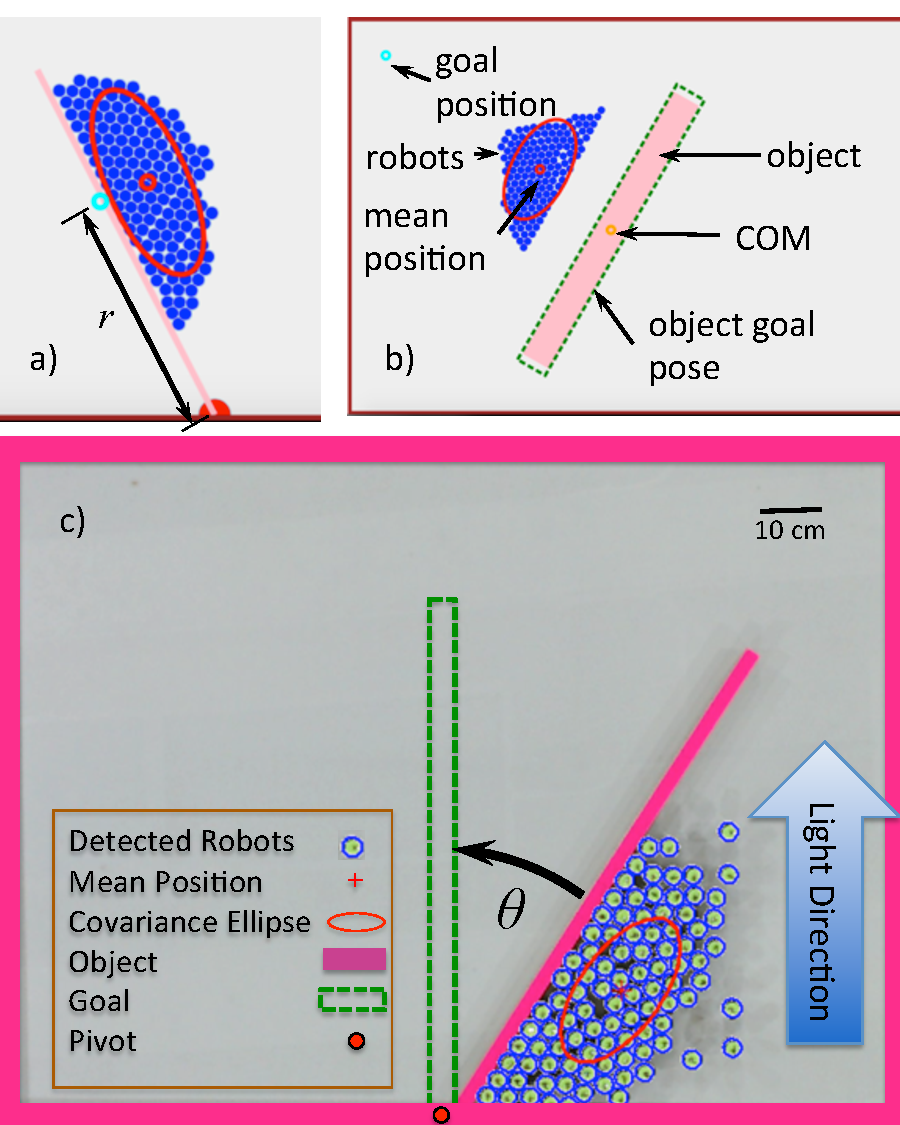
\includegraphics[width=.9\columnwidth]{CoverPhoto.pdf}
\end{center}
\vspace{-1em}
\caption{\label{fig:FirstImage}
%Torque control of an object is essential for manipulation unless objects are homogeneous discs, especially when there are narrow passageways or the objects must be aligned, e.g. sensors and emitters. 
%This paper provides the optimal position for a swarm to push to maximize torque production using a highly under-actuated system where all robots are controlled uniformly by the same input. 
(a) Simulation of robots exerting torque on a hinged ``door".
(b) Orientation control of a free long rod.
(c) Hardware robots applying torque to an object. See video attachment.% A full resolution video is available at \url{https://youtu.be/7Q5lu_ZFbxI}.
}
\vspace{-1em}
\end{figure}

With a single agent, torque control is straightforward: the agent simply maximizes the length of the movement arm to maximize torque. To make an agent push open a door, it should push on the edge furthest from the hinge. 
The optimal solution for a swarm of particles is not straightforward because they cannot all push at one position.

This chapter focuses on maximizing torque using the swarm's position distribution. 
Representative results are shown in Fig. \ref{fig:FirstImage}:  torque control using 56 mobile robots on a pivoted and a free object.



